\documentclass[tikz,border=10pt]{standalone}

\usepackage{tikz}
\usetikzlibrary{positioning}
\usetikzlibrary{shapes,arrows,backgrounds,fit,shapes.geometric,calc}
\usetikzlibrary{pgfplots.groupplots}
\usetikzlibrary{patterns}
\usepackage{pgfplots}
\usepackage{pgfplotstable}
\usepackage{listings}
\usepackage{lstautogobble}
\usepackage{color}

\renewcommand{\familydefault}{\sfdefault}

\begin{document}
\tikzset{>=stealth', pil/.style={ ->, color=black!60, thick, } }
\begin{figure}
    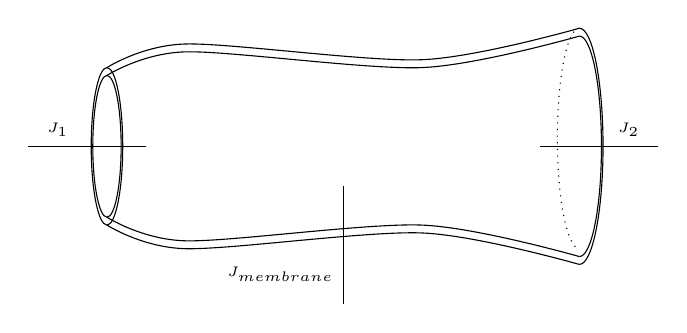
\begin{tikzpicture}%[scale=0.6]
	\foreach \r in {-1,1}
	    \foreach \y in {0,-0.1cm}
		\draw[yscale=\r] plot[smooth,yshift=\y] coordinates{(0,1) (1,1.3) (4,1.1) (6,1.5)};
	\draw (0,0) ellipse [x radius=0.2cm, y radius=1cm];
	\draw (0,0) ellipse [x radius=0.18cm, y radius=0.9cm];
	\draw (6,-1.5) arc [start angle=-90, end angle=90, x radius=0.3cm, y radius=1.5cm];
	\draw (6,-1.4) arc [start angle=-90, end angle=90, x radius=0.28cm, y radius=1.4cm];
	\draw[dotted] (6,1.5) arc [start angle=90, end angle=270, x radius=0.28cm, y radius=1.4cm];
	\draw (0.5,0) -- node[above, near end] {\tiny $J_1$} (-1,0);
	\draw (7,0) -- node[above, near start] {\tiny $J_2$} (5.5,0);
	\draw (3,-0.5) -- node[left, near end] {\tiny $J_\text{membrane}$} (3,-2);
    \end{tikzpicture}
    \caption{Current balance in dendrite section, $J_\text{membrane}=J_2-J_1$.
	The membrane is treated as a leaky capacitor
	with extra current sources, surrounding an ohmic conductor of variable radius.}
    \label{fig:currentbalance}
\end{figure}
\end{document}

